\section{Proof of Concept Attacks}
The previous section (Section. \ref{Arch:Test}) discussed in detail how we verified that our system functions according to our expectations. This section describes how we validated our expectations. In order to do this, we constructed three sets of web applications in PHP, Python, and Ruby. Each of these applications was a simple web app that took in user input to construct and send an E-Mail.

The front-end for each of the three applications is shown in Listing. \ref{code:html}. The back-end for the three languages are shown in Listings \ref{code:phpemi}, \ref{code:pyemi}, and \ref{code:rubyemi}.

We tested for the headers being injected in real-time by running an instance of MailCatcher, set to listen on all SMTP messages. A sample screenshot of a fuzzed request for the Ruby backend (generated in PostMan) is shown in Figure~\ref{fig:postmanruby}. The E-Mail sent due to injecting this payload (as captured by MailCatcher) is shown in Figure~\ref{fig:mailcatcherruby}. It can be seen that the Headers have been added to the resulting E-Mail, and we have successfully managed to overwrite the `Subject' field with our message, `hello'.

A similar injection example for PHP is shown in Figure~\ref{fig:postmanphp} and the corresponding E-Mail caught by MailCatcher is shown in Figure~\ref{fig:mailcatcherphp}. The astute reader might have noticed that in the given examples we have used `\%0a' to separate the headers, while in Section. \ref{Comp:Fuzzer:mp}, we had used `\textbackslash{}n'. This is due to URL Encoding (\cite{rfc1738}), wherein special characters are `encoded' or `escaped' with their ASCII equivalent.
The reason why we do not have to do this with the payloads our system injects is due to the fact that the `Requests' library that we use to generate the HTTP requests automatically does this encoding for us.

\lstset{language=HTML,caption={HTML page for showcasing e-mail header injection, a simple front-end for our examples.},label={code:html}}
\begin{lstlisting}
<!doctype html>
<html lang="en">
<head>
<meta charset="utf-8">
<meta name="author" content="Sai Pc">
<title>Mock Email</title>
</head>
<body>
<form action="{Replace with path to back-end}" method="post">
<input type="text" placeholder="Email" name="email" id="e-mail"><br>
<textarea name="msg" rows="20" cols="120"></textarea>
<input type="submit" value="Email Me!">
</form>
</body>
</html>
\end{lstlisting}

\begin{figure}[!htbp]
	\centering
	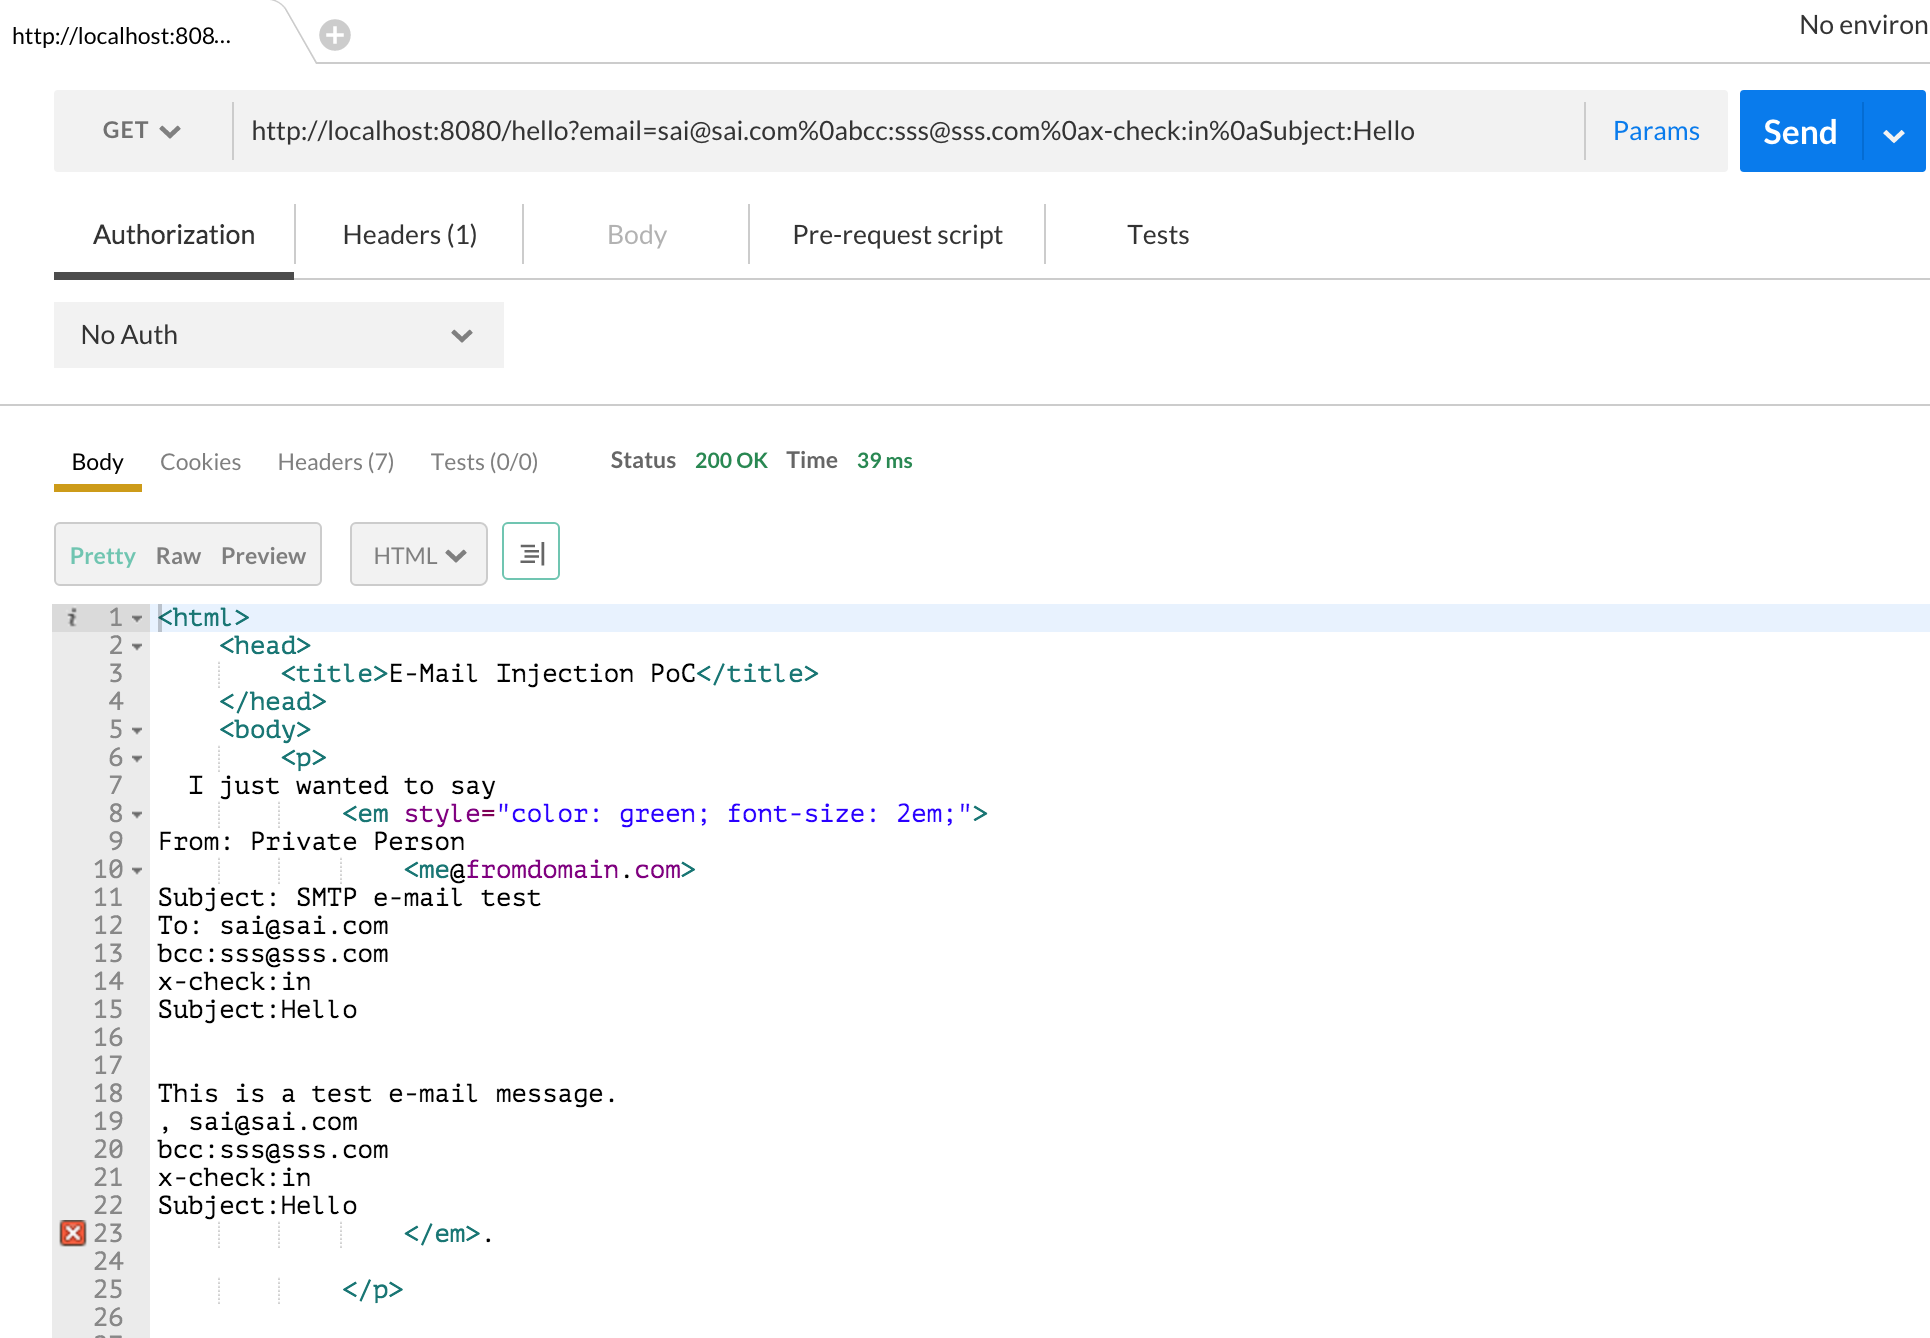
\includegraphics[width=14cm, height=8cm]{System/EMI_Postman_Ruby}
	\caption[Fuzzing a request for the ruby backend]{Fuzzing a request for the ruby backend, the payload can be seen inside the address bar on top.}
	\label{fig:postmanruby}
\end{figure}

\begin{figure}[!htbp]
	\centering
	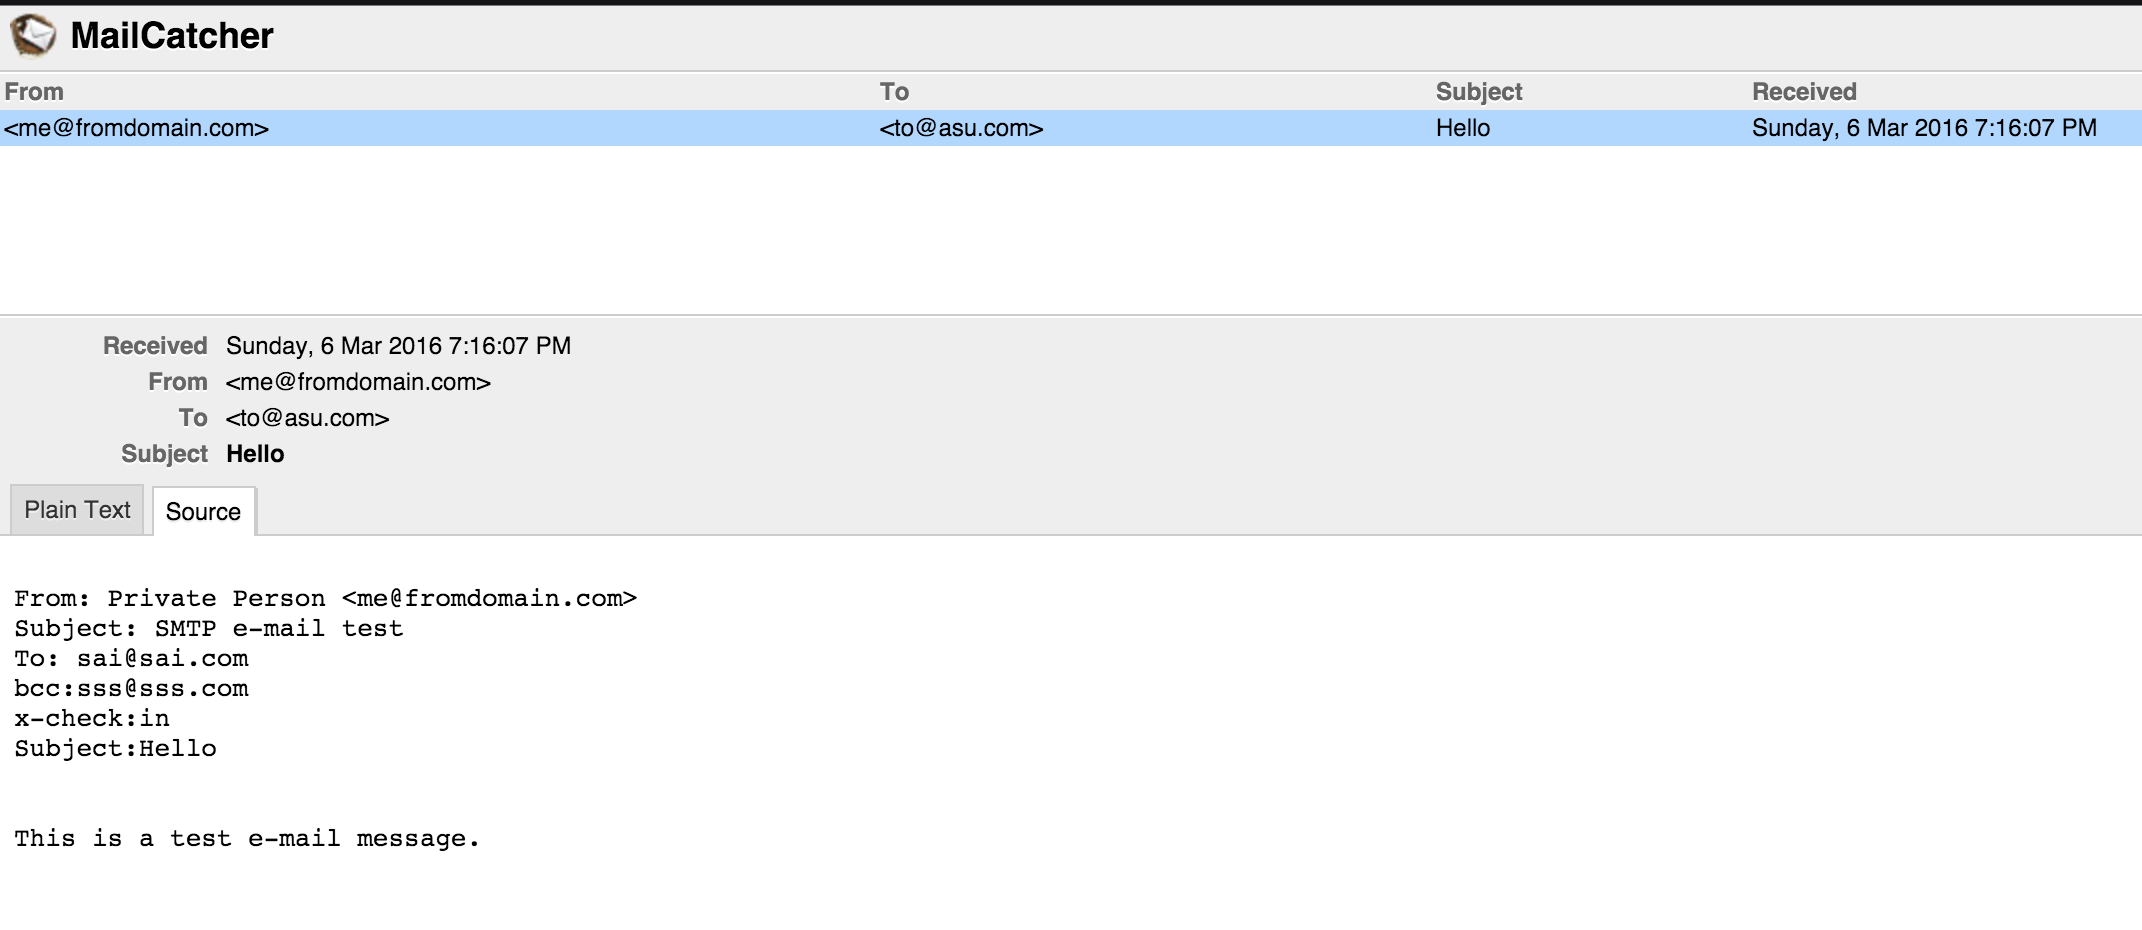
\includegraphics[width=14cm, height=8cm]{System/EMI_Mailcatcher_Ruby}
	\caption[E-Mail header injection proof of concept - ruby]{E-Mail header injection proof of concept - ruby, we can see that multiple headers (bcc, x-check, Subject) have been inserted into the resulting e-mail.}
	\label{fig:mailcatcherruby}
\end{figure}

\begin{figure}[!htbp]
	\centering
	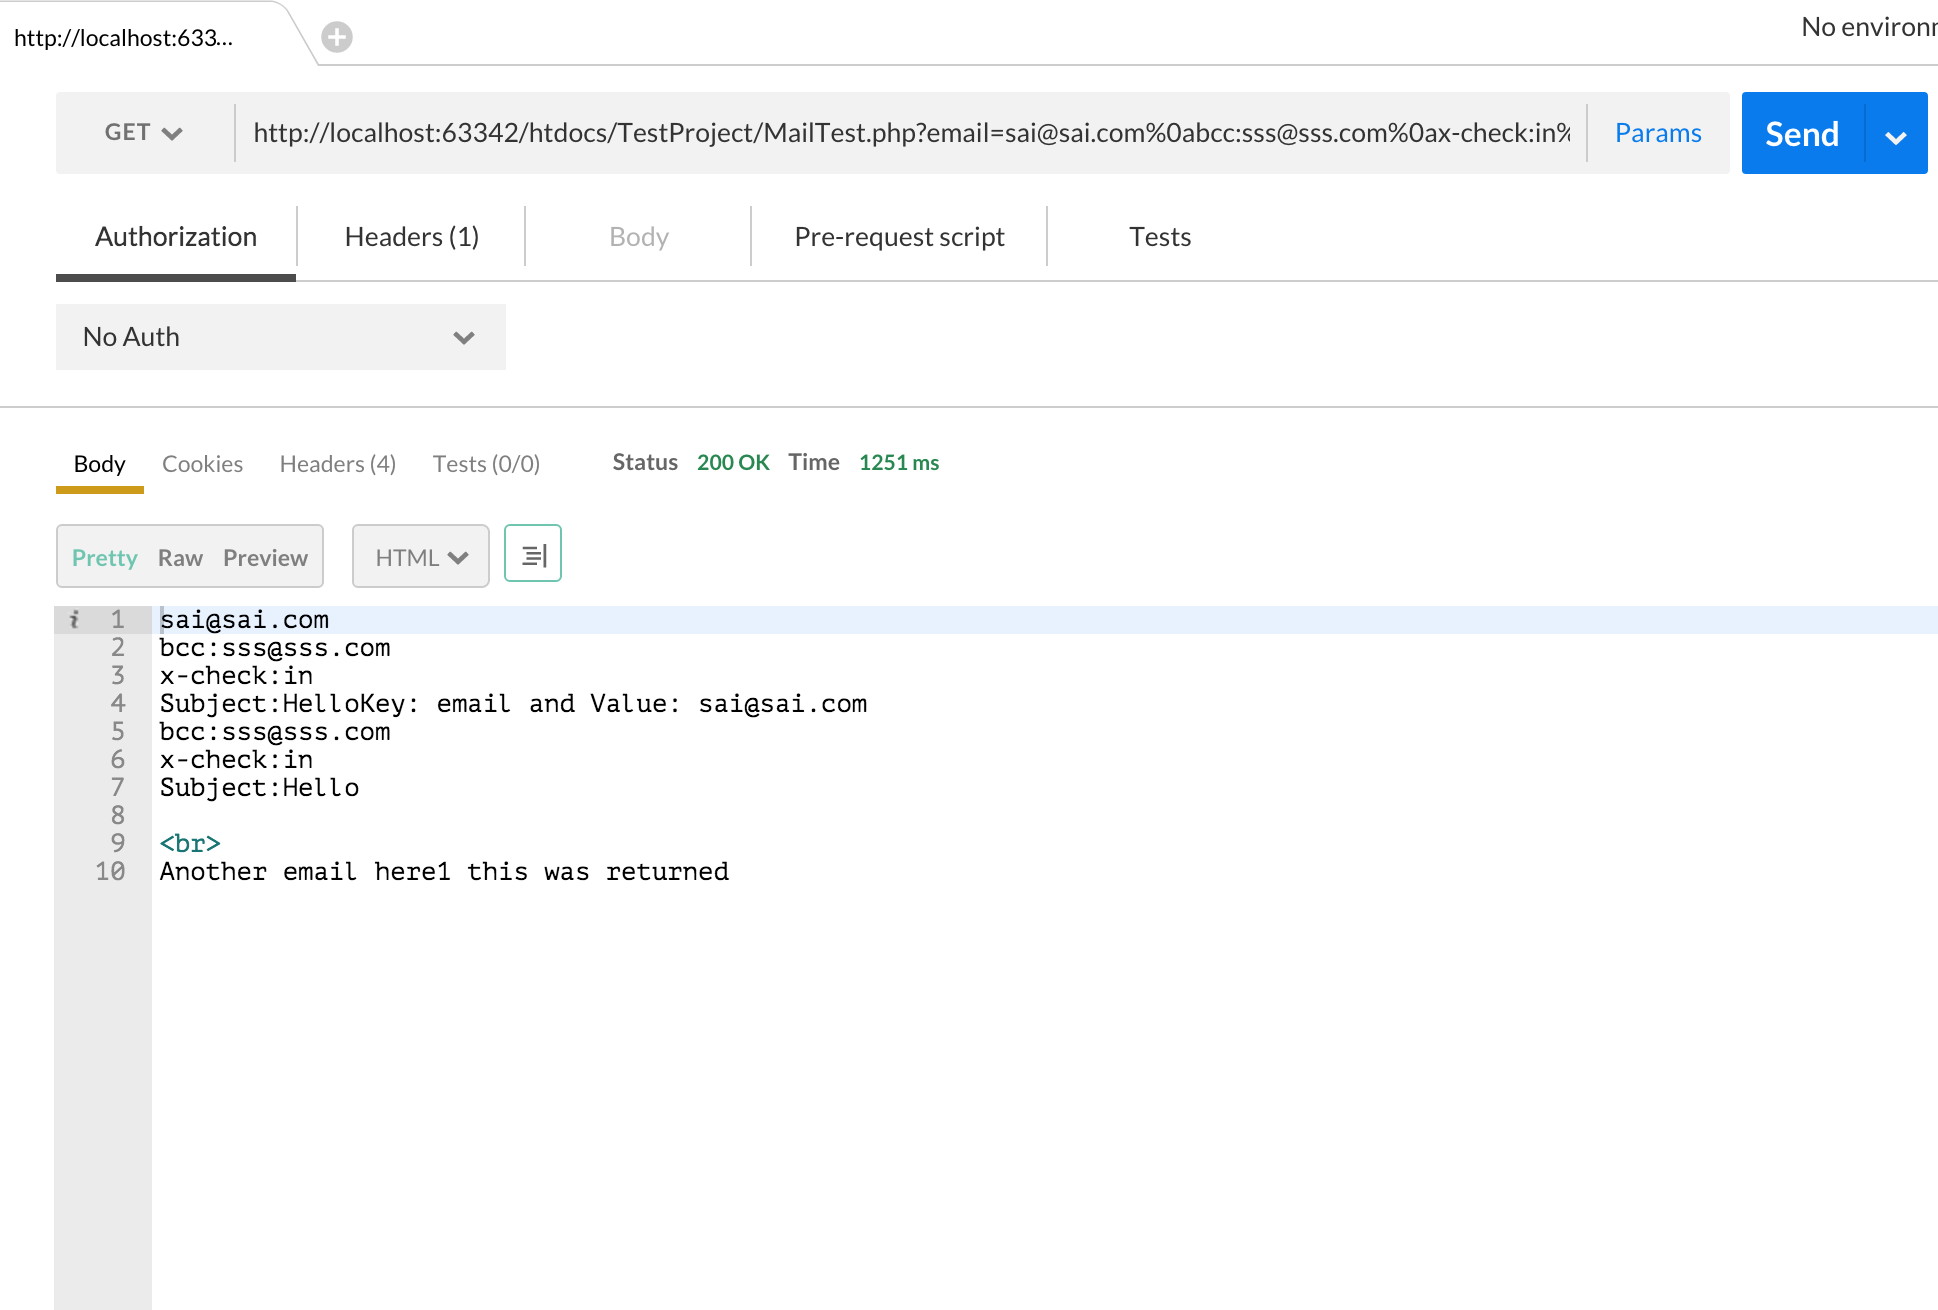
\includegraphics[width=14cm, height=8cm]{System/EMI_Postman_PHP}
	\caption[Fuzzing a request for the php backend]{Fuzzing a request for the php backend, the payload can be seen inside the address bar on top.}
	\label{fig:postmanphp}
\end{figure}

\begin{figure}[!htbp]
	\centering
	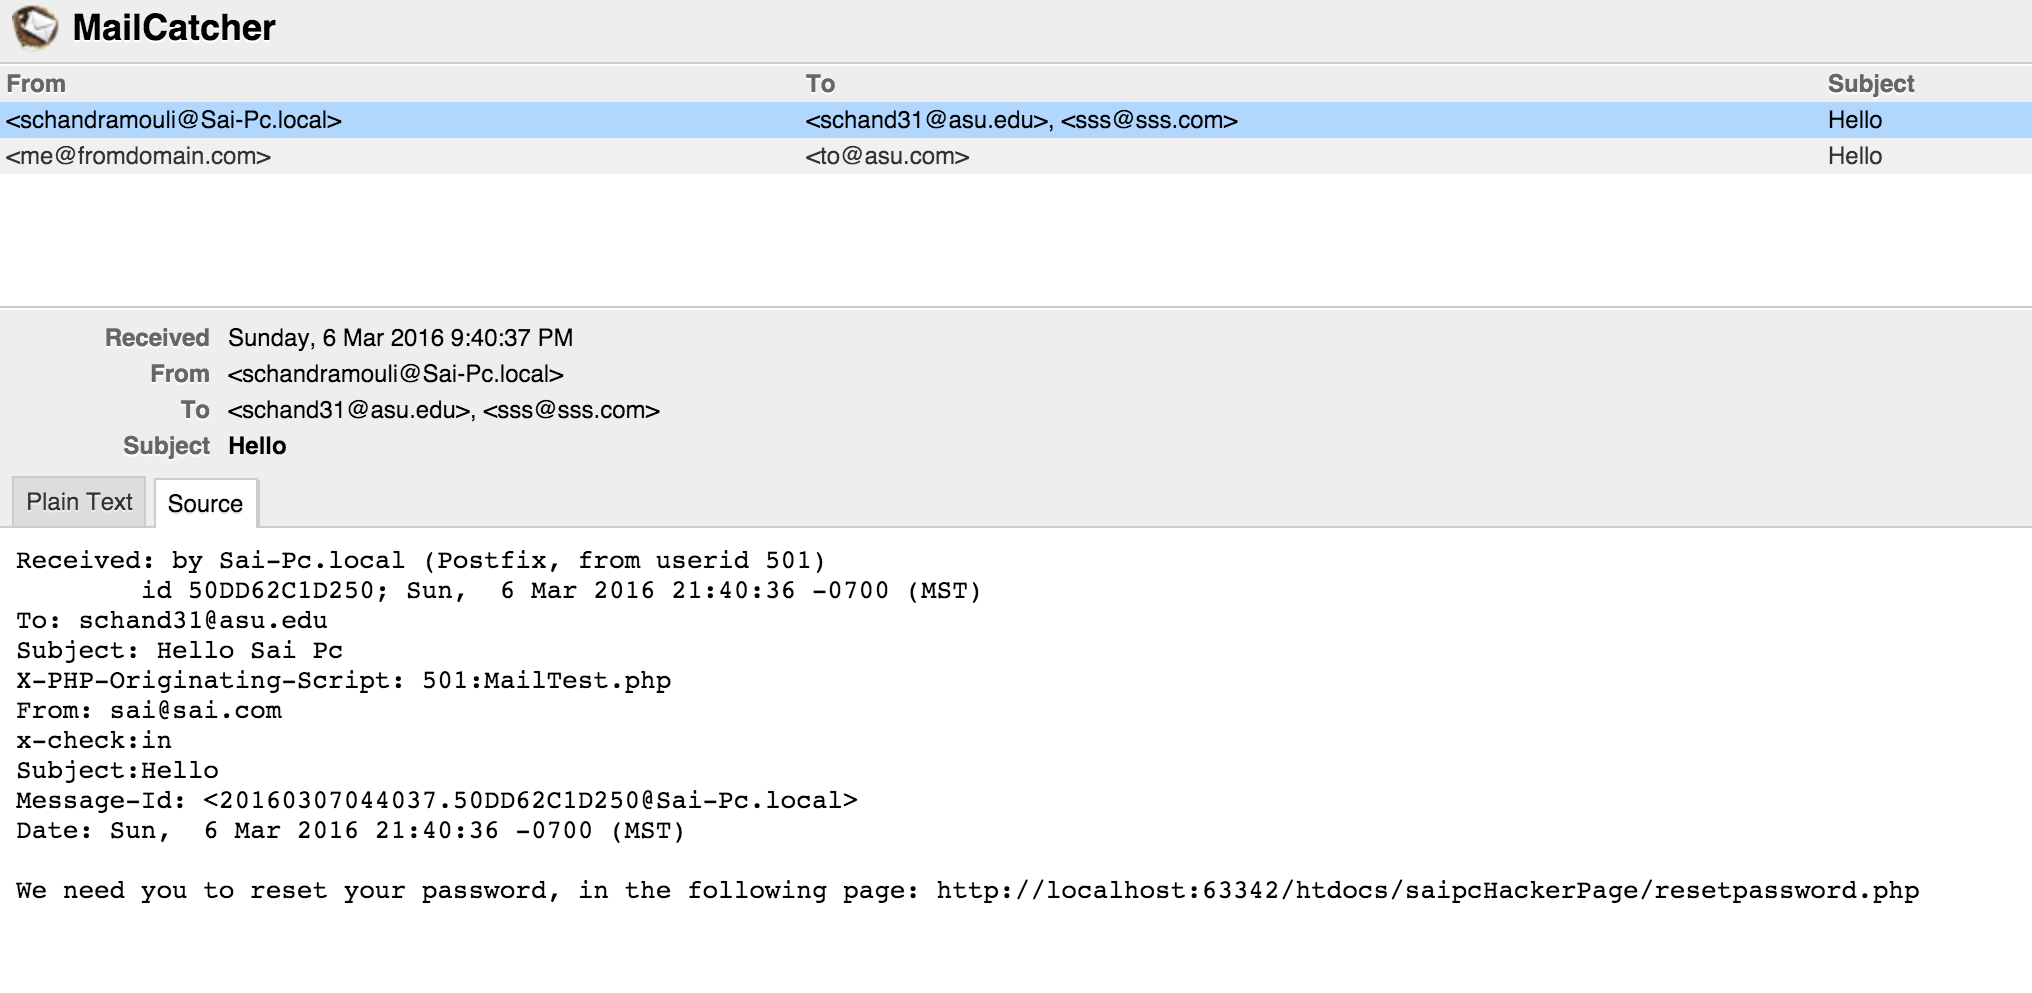
\includegraphics[width=14cm, height=8cm]{System/EMI_Mailcatcher_PHP}
	\caption[E-Mail header injection proof of concept - php]{E-Mail header injection proof of concept - php, we can see that multiple headers (bcc, x-check, Subject) have been inserted into the resulting e-mail.}
	\label{fig:mailcatcherphp}
\end{figure}